
\setcounter{demsode}{4} %%% THỨ TỰ ĐỀ THẦY - CÔ ĐÃ NHẬN

\begin{name}
	{Biên soạn: Dương Công Tạo\\
	Phản biện: Hải Phụng}
	{ÔN TẬP HỌC KỲ II KHỐI 10 NĂM 2024}
\end{name}

\cautn
\Opensolutionfile{ans}[ans/0-CTST-TN-SO-4]
\setcounter{ex}{0}
%%%=============EX_1=============%%%
\begin{ex}%[DA-HK2-K10,11-2024 - Dương Công Tạo]%[0H9N3-1]
	Cho đường thẳng $\Delta\colon 2x-y+1=0$. Điểm nào sau đây nằm trên đường thẳng $\Delta$?
	\choice
	{\True $B\left(\dfrac{1}{2};2\right)$}
	{$C\left(\dfrac{1}{2};-2\right)$}
	{$D(0;-1)$}
	{$A(1;1)$}
	\loigiai{
		
	}
\end{ex}

%%%=============EX_2=============%%%
\begin{ex}%[DA-HK2-K10,11-2024 - Dương Công Tạo]%[0D0N1-3]
	Rút ngẫu nhiên cùng lúc ba con bài từ cỗ bài tú lơ khơ $52$ con thì $n(\Omega)$ bằng bao nhiêu?
	\choice
	{$140\,608$}
	{$156$}
	{$132\,600$}
	{\True $22\,100$}
	\loigiai{
		
	}
\end{ex}

%%%=============EX_3=============%%%
\begin{ex}%[DA-HK2-K10,11-2024 - Dương Công Tạo]%[0H9N3-1]
	Tìm tọa độ vectơ chỉ phương của đường thẳng đi qua $2$ điểm $A(2; 2)$ và $B(1; 0)$?
	\choice
	{$(2;-1)$}
	{$(4; 2)$}
	{$(-1; 2)$}
	{\True $(1;2)$}
	\loigiai{
		
	}
\end{ex}

%%%=============EX_4=============%%%
\begin{ex}%[DA-HK2-K10,11-2024 - Dương Công Tạo]%[0D7H2-1]
	Tập xác định của hàm số $y=\sqrt{2x^2-5x+2}$ là
	\choice
	{\True $\left(-\infty; \dfrac{1}{2}\right] \cup[2;+\infty)$}
	{$\left(\dfrac{1}{2}; 2\right)$}
	{$\left(-\infty; \dfrac{1}{2}\right) \cup(2;+\infty)$}
	{$\left[\dfrac{1}{2}; 2\right]$}
	\loigiai{
	
	}
\end{ex}

%%%=============EX_5=============%%%
\begin{ex}%[DA-HK2-K10,11-2024 - Dương Công Tạo]%[0D7H1-2]
	Dấu của tam thức bậc hai $f(x)=-x^2+5x-6$ được xác định như sau
	\choice
	{$f(x) < 0$ với $2< x < 3$ và $f(x) > 0$ với $x < 2$ hoặc $x > 3$}
	{$f(x) < 0$ với $-3< x <-2$ và $f(x) > 0$ với $x <-3$ hoặc $x >-2$}
	{\True $f(x) > 0$ với $2< x < 3$ và $f(x) < 0$ với $x < 2$ hoặc $x > 3$}
	{$f(x) > 0$ với $-3< x <-2$ và $f(x) < 0$ với $x <-3$ hoặc $x >-2$}
	\loigiai{
	
	}
\end{ex}

%%%=============EX_6=============%%%
\begin{ex}%[DA-HK2-K10,11-2024 - Dương Công Tạo]%[0D0H2-2]
	Gieo một con súc sắc cân đối đồng chất một lần. Tính xác suất để xuất hiện mặt có số chấm là một số nguyên tố.
	\choice
	{\True $\dfrac{1}{3}$}
	{$\dfrac{1}{4}$}
	{$\dfrac{1}{2}$}
	{$\dfrac{2}{3}$}
	\loigiai{
		
	}
\end{ex}

%%%=============EX_7=============%%%
\begin{ex}%[DA-HK2-K10,11-2024 - Dương Công Tạo]%[0D8N1-1]
	Trên giác sách có $10$ quyển sách Tiếng Việt khác nhau, $8$ quyển sách Tiếng Anh khác nhau và $5$ quyển sách Tiếng Pháp khác nhau. Hỏi có bao nhiêu cách chọn một quyễn sách không là sách Tiếng Việt?
	\choice
	{\True $13$}
	{$40$}
	{$23$}
	{$400$}
	\loigiai{
	
	}
\end{ex}

%%%=============EX_8=============%%%
\begin{ex}%[DA-HK2-K10,11-2024 - Dương Công Tạo]%[0H9N3-2]
	Trong mặt phẳng $Ox y$, đường thẳng đi qua điểm $A(2;-4)$ và nhận $\vec{u}=(-4; 3)$ là vec-tơ chỉ phương có phương trình tham số là
	\choice
	{$\dfrac{x-2}{-4}=\dfrac{y+4}{3}$}
	{$\heva{&x=-4+2t \\
			&y=3-4t
			&}$}
	{\True $\heva{&x=2-4t \\
			&y=-4+3t
			&}$}
	{$\heva{&x=-2-4t \\
			&y=4+3t
			&}$}
	\loigiai{
	
	}
\end{ex}

%%%=============EX_9=============%%%
\begin{ex}%[DA-HK2-K10,11-2024 - Dương Công Tạo]%[0D7H3-2]
	Số nghiệm của phương trình $\sqrt{x^2-2x+5}=x^2-2x+3$ là
	\choice
	{$2$}
	{$3$}
	{\True $1$}
	{$0$}
	\loigiai{
	
	}
\end{ex}

%%%=============EX_10=============%%%
\begin{ex}%[DA-HK2-K10,11-2024 - Dương Công Tạo]%[0H9H4-4]
	Cho đường tròn $(C)\colon x^2+y^2-4x+2y-7=0$ và hai điểm $A(1; 1), B(-1; 2)$. Khẳng định nào dưới đây đúng?
	\choice
	{$A$ và $B$ cùng nằm trong $(C)$}
	{\True $A$ nằm trong và $B$ nằm ngoài $(C)$}
	{$A$ và $B$ cùng nằm ngoài $(C)$}
	{$A$ nằm ngoài và $B$ nằm trong $(C)$}
	\loigiai{
		
	}
\end{ex}

%%%=============EX_11=============%%%
\begin{ex}%[DA-HK2-K10,11-2024 - Dương Công Tạo]%[0D8H1-3]
	Bình có $5$ cái áo khác nhau, $4$ chiếc quần khác nhau, $3$ đôi giầy khác nhau và $2$ chiếc mũ khác nhau. Số cách chọn một bộ gồm quần, áo, giầy và mũ của Bình là
	\choice
	{$14$}
	{\True $120$}
	{$60$}
	{$5$}
	\loigiai{
		
	}
\end{ex}

%%%=============EX_12=============%%%
\begin{ex}%[DA-HK2-K10,11-2024 - Dương Công Tạo]%[0D8N2-2]
	Cần chọn $3$ người đi công tác từ một tổ có $30$ người, khi đó số cách chọn là
	\choice
	{$\mathrm{A}_{30}^3$}
	{$3^{30}$}
	{$10$}
	{\True $\mathrm{C}_{30}^3$}
	\loigiai{
	
	}
\end{ex}
\Closesolutionfile{ans}
\indapan{6}{ans/0-CTST-TN-SO-4}

\cauds
\Opensolutionfile{ans}[ans/0-CTST-DS-SO-4]
\setcounter{ex}{0}

%%%============EX_1==============%%%
\begin{ex}%[DA-HK2-K10,11-2024 - Dương Công Tạo]
	Trong hộp bút của Lan có $4$ chiếc bút chì, $5$ chiếc bút bi và $2$ chiếc bút máy (tất cả đều khác nhau), khi đó:
	\choiceTF
	{\True Số cách chọn $1$ chiếc bút chì và $1$ chiếc bút bi là $20$ (cách)}
	{Số cách chọn $1$ chiếc bút chì và $1$ chiếc bút máy là $4$ (cách)}
	{Số cách chọn $1$ chiếc bút bi và $1$ chiếc bút máy là $7$ (cách)}
	{\True Số cách chọn $2$ chiếc bút khác loại với nhau từ hộp bút của Lan là $38$ (cách)}
	\loigiai{
	
	}
\end{ex}

%%%============EX_2==============%%%
\begin{ex}%[DA-HK2-K10,11-2024 - Dương Công Tạo]
	Cho biểu thức $f(x)=(3x-1)\left(3x^2-4x+1\right)$. Khi đó
	\choiceTF
	{\True $f(x)=0\Leftrightarrow\hoac{&x=-\dfrac{1}{3} \\&x=1&}$}
	{\True Với $x \in\left(-\infty; \dfrac{1}{3}\right) \cup\left(\dfrac{1}{3}; 1\right)$ thì $f(x) < 0$}
	{Với $x \in(1;+\infty)$ thì $f(x) < 0$}
	{\True Bảng xét dấu của biểu thức là \\
		\begin{tikzpicture}
				\tkzTabInit[lgt=3,espcl=2]
				{$x$/0.7,$3x-1$/0.7,$3x^2-4x+1$/0.7,$f(x)$/.7}
				{$-\infty$,$\tfrac{1}{3}$,$1$,$+\infty$}
				\tkzTabLine{,-,t,+,z,+,}
				\tkzTabLine{,+,z,-,z,+,}
				\tkzTabLine{,-,z,-,z,+,}
			\end{tikzpicture}
		}
	\loigiai{
	
	}
\end{ex}

%%%============EX_3==============%%%
\begin{ex}%[DA-HK2-K10,11-2024 - Dương Công Tạo]
	Cho biểu thức $f(x)=\dfrac{1}{x^2-2x-12}$. Khi đó:
	\choiceTF
	{$f(x)=0\Leftrightarrow x=1+\sqrt{13}$ hoặc $x=1-\sqrt{13}$}
	{Với $x \in(1-\sqrt{13}; 1+\sqrt{13})$ thì $f(x) > 0$}
	{Với $x \in(-\infty; 1-\sqrt{13}) \cup(1-\sqrt{13};+\infty)$ thì $f(x) < 0$}
	{\True Bảng xét dấu của biểu thức là\\
		
\begin{tikzpicture}
			\tkzTabInit[lgt=3,espcl=2]
			{$x$/0.7,$x^2-2x-12$/0.7,$f(x)$/.7}
			{$-\infty$,$1-\sqrt{13}$,$1-\sqrt{13}$,$+\infty$}
			\tkzTabLine{,+,z,-,z,+,}
			\tkzTabLine{,+,d,-,d,+,}
		\end{tikzpicture}}
	\loigiai{
		
	}
\end{ex}

%%%============EX_4==============%%%
\begin{ex}%[DA-HK2-K10,11-2024 - Dương Công Tạo]
	Cho số tự nhiên $\overline{a b c d e}$ với $a, b, c, d, e$ là các số lấy từ tập $\{0; 1; 2; 3; 4; 5; 6; 7; 8; 9\}$, khi đó:
	\choiceTF
	{Có $100\,000$ số}
	{\True Có $27\,216$ số mà các chữ số $a, b, c, d, e$ đôi một khác nhau}
	{\True Có $13\,440$ số mà các chữ số $a, b, c, d, e$ đôi một khác nhau và số tự nhiên đó là số lẻ}
	{\True Có $13\,776$ số mà các chữ số $a, b, c, d, e$ đôi một khác nhau và số tự nhiên đó chẵn}
	\loigiai{
		
	}
\end{ex}

\Closesolutionfile{ans}
\indapan{4}{ans/0-CTST-DS-SO-4}

\caukq
\Opensolutionfile{ans}[ans/0-CTST-KQ-SO-4]
\setcounter{ex}{0}

%%%=============EX_1=============%%%
\begin{ex}%[DA-HK2-K10,11-2024 - Dương Công Tạo]
	Giải bất phương trình $\left(x^2-3x+2\right)\left(-x^2+5x-6\right) \geq 0$ ta được tập nghiệm là $S=[a;b]$. Khi đó tổng $a+b$ bằng
	\shortans[]{$4$}
	\loigiai{
		
	}
\end{ex}

%%%=============EX_2=============%%%
\begin{ex}%[DA-HK2-K10,11-2024 - Dương Công Tạo]
	Có bao nhiêu giá trị nguyên của tham số $m$ để bất phương trình $x^2+2m x+m-2< 0$ nghiệm đúng với mọi $x \in(1; 2)$.
	\shortans[]{$1$}
	\loigiai{
	
	}
\end{ex}

%%%=============EX_3=============%%%
\begin{ex}%[DA-HK2-K10,11-2024 - Dương Công Tạo]
	Một chú thỏ đen chạy đuổi theo một chú thỏ trắng ở vị trí cách nó $100$ m. Biết rằng, quãng đường chú thỏ đen chạy được biểu thị bởi công thức $s(t)=8t+5t^2$ (m), trong đó $t$ (giây) là thời gian tính từ thời điểm chú thỏ đen bắt đầu chạy, và chú thỏ trắng chạy với vận tốc không đổi là $3$ m/s. Để chú thỏ đen chạy trước chú thỏ trắng thì giá trị nguyên dương nhỏ nhất của $t$ là bao nhiêu?
	\shortans[]{$5$}
	\loigiai{
	
	}
\end{ex}

%%%=============EX_4=============%%%
\begin{ex}%[DA-HK2-K10,11-2024 - Dương Công Tạo]
	Bộ phận nghiên cứu thị trường của một xí nghiệp xác định tổng chi phí để sản xuất $Q$ sản phẩm là $Q^2+3\,00Q+200\,000$ (nghìn đồng). Giả sử giá mỗi sản phẩm bán ra thị trường là $1\,200$ nghìn đồng. Hỏi xí nghiệp cần sản xuất tối thiểu bao nhiêu sản phẩm thì không bị lỗ?
	
	\shortans[]{$400$}
	\loigiai{
	
	}
\end{ex}

%%%=============EX_5=============%%%
\begin{ex}%[DA-HK2-K10,11-2024 - Dương Công Tạo]
	\immini{Cho tam giác $ABC$ có cạnh $BC=10$, góc $\widehat{ABC}=60^{\circ}$ và $AB<BC$. Trên cạnh $AB$ ta lấy điểm $M$ sao cho $AM=3$ (như hình vẽ).
		Tính độ dài đoạn thẳng $BM$ biết rằng $CM=\dfrac{8}{9} CA$ (đáp số gần đúng đến hàng phần trăm).}
	{
\begin{tikzpicture}[font=\footnotesize]
	\def\a{2}
	\path 	(0:0) coordinate (B)
			(0:\a) coordinate (C)
			(60:1.5*\a) coordinate (A)
			($(B)+(70:\a)$) coordinate (A)
			($(A)!.3!(B)$) coordinate (M);
	\draw	(A)--(M)node[pos=0.9,sloped,above,rotate=-60]{$3$}--(B)--(C)node[pos=0.5,sloped,above]{$10$}--cycle
					(C)--(M);
	\foreach \x/\g in {A/90,B/180,C/0,M/170}
			\fill[black] 	(\x) circle (1pt)
			($(\g:4mm)+(\x)$) node {$\x$};
\end{tikzpicture}}
	\shortans[]{$6$}
	\loigiai{
	
	}
\end{ex}

%%%=============EX_6=============%%%
\begin{ex}%[DA-HK2-K10,11-2024 - Dương Công Tạo]
	Trong mặt phẳng tọa độ $Oxy$, cho tam giác $ABC$. Gọi $AM$, $AD$ lần lượt là đường trung tuyến và đường phân giác trong của tam giác. Các đường thẳng $AM$, $AD$ lần lượt có phương trình trình là $x-y-2=0$; $y=0$. Giả sử $B(1;3)$. Khi đó, đường thẳng $AC$ có dạng $ax+by+c=0$ và tọa độ điểm $C\left(d;e\right)$. Giá trị biểu thức $O=a+b+c+d+e$ bằng
	\shortans[]{$-10$}
	\loigiai{
		
	}
\end{ex}
\Closesolutionfile{ans}
\indapan{6}{ans/0-CTST-KQ-SO-4}